% Intended LaTeX compiler: pdflatex
\documentclass[10pt,a4paper,UTF8]{article}
\usepackage{zclorg}
\usepackage{tikztheorem}
\author{emacsun}
\date{}
\title{神经网络要点理解}
\hypersetup{
 pdfauthor={emacsun},
 pdftitle={神经网络要点理解},
 pdfkeywords={},
 pdfsubject={},
 pdfcreator={Emacs 25.0.50.1 (Org mode 9.1.2)},
 pdflang={English}}
\begin{document}

\maketitle
\tableofcontents
\titlepic{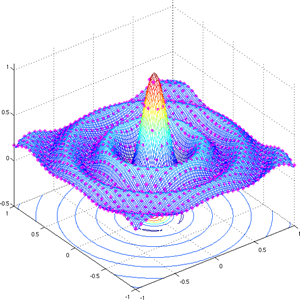
\includegraphics[scale=0.25]{../../img/sinc.PNG}}
第一次接触神经网络总是被其诸多的符号弄的眼花缭乱。几个重要的符号包括:

\begin{enumerate}
\item 样本的个数\(m\);
\item 单个样本的feature个数\(n\);
\item 神经网络的层数\(L\);
\item 神经网络输出的类别数量\(K\);
\end{enumerate}

假设我们对5000幅\(20\times 20\)的手写数字灰度图像进行识别,则\(m=5000,n=400,K=10\)。对于本文用到的神经网络,\(L=3\)。

\section{损失函数及其正则化}
\label{sec:org8860247}
一个未经正则化的神经网络损失函数为:
\begin{equation}
\label{eq:1}
J(\Theta) = \frac{1}{m} \sum_{i=1}^{m} \sum_{k=1}^{K} \big[ - y_{k}^{(i)}\log ((h_{\theta}(x^{(i)}))_{k}) - (1-y_{k}^{(i)})\log (1- (h_{\theta}(x^{(i)}))_{k} ) \big]
\end{equation}

其中\(h_{\theta}(x)\)的计算如下:

\begin{center}
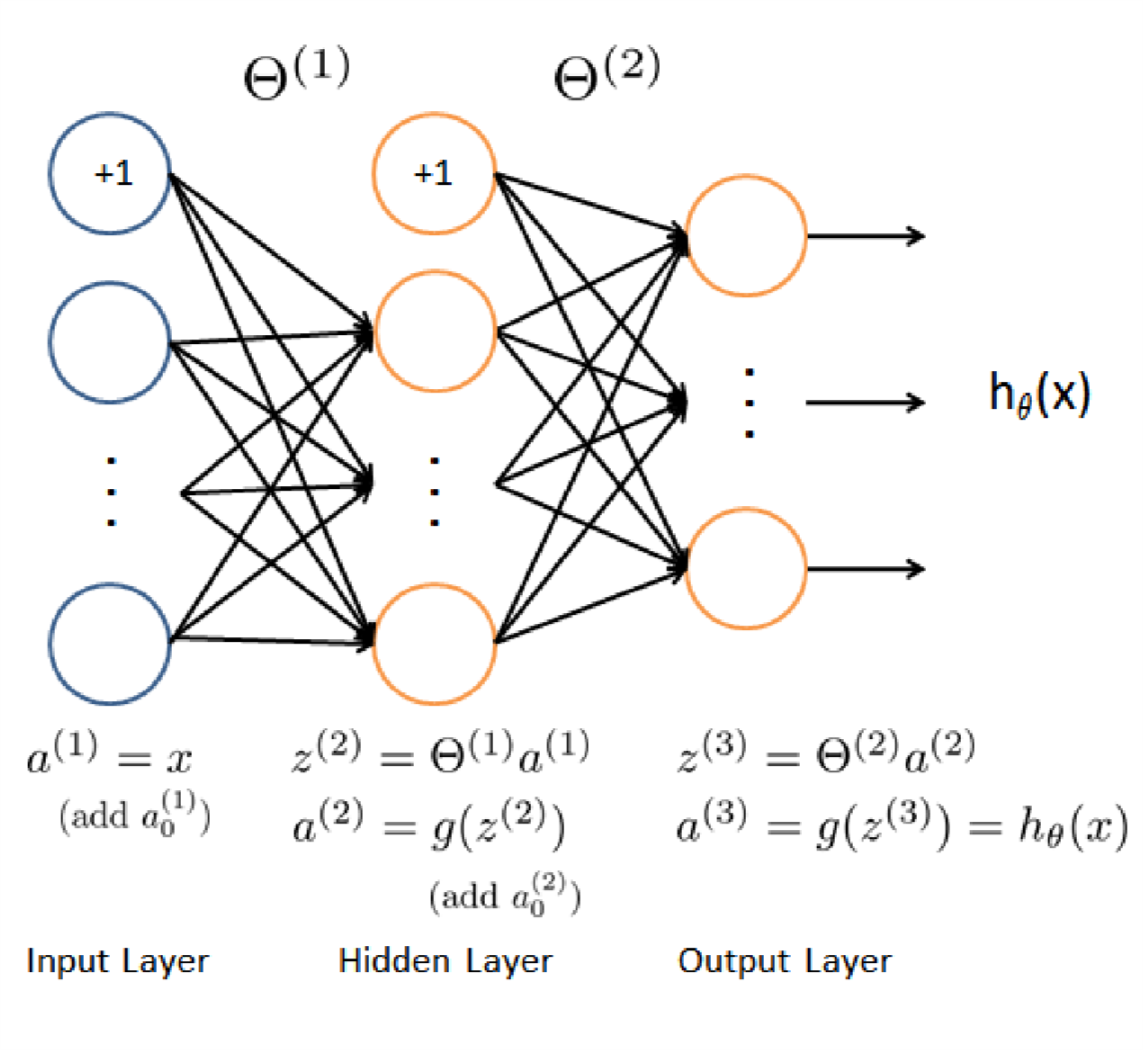
\includegraphics[width=.9\linewidth]{../../img/computer_ng/20171014htheta.png}
\end{center}

此处\(L=3\).

针对上面的公式,我们有\(x^{(i)}\)表示第\(i\)个样本的矢量,这个矢量的大小是\(400\times 1\)。\(h_{\theta}(x^{(i)})_{k}\)表示第\(i\)个输入在第\(K\)个类上的输出。每一个输入样本\(x^{(i)}\)都会在神经网络的输出层产生\(K\)个输出,表示\(x^{(i)}\)属于这\(K\)个类中每个类的可能性。

当我们给定\(\Theta_{1}\),\(\Theta_{2}\)时,我们可以根据上图来计算每一个\(h_{\theta}(x^{i})\),进而根据\(J(\Theta)\)的公式来计算损失函数。

注意在计算的过程中,我们遇到的一些矩阵(从上图到\(J(\Theta)\)的计算过程中遇到的矩阵)的维度为:

\begin{center}
\begin{tabular}{ll}
矩阵 & 维度\\
\hline
\(a^{(1)}\) & \(5000\times 401\)\\
\(\Theta^{(1)}\) & \(25\times 401\)\\
\(z^{(2)}\) & \(25\times 5000\)\\
\(a^{(2)}\) & \(26\times 5000\)\\
\(\Theta^{(2)}\) & \(10\times 26\)\\
\(z^{(3)}\) & \(10\times 5000\)\\
\(a^{(3)}\) & \(10\times 5000\)\\
\(Y\) & \(10\times 5000\)\\
\end{tabular}
\end{center}

其中\(a^{(1)}\) 为添加了\(a_{0}^{(1)}\)后的矩阵;\(a^{(2)}\)为添加了\(a_{0}^{(2)}\)后的矩阵;\(Y\)为把1,2,\ldots{},10映射为矢量后的矩阵。


\(J(\Theta)\)计算的是5000个用户在10个类上的cost之和。所以式\textasciitilde{}(\ref{eq:1})的方括号中如果是矩阵的话应该是一个\(10\times 5000\)的矩阵。

计算\(J(\Theta)\)的部分代码为:
\lstset{language=matlab,label= ,caption= ,captionpos=b,numbers=none}
\begin{lstlisting}
a1 = [ones(m,1) X];
z2 = Theta1*a1';
a2 = 1./(1 + exp(-z2));
a2 = [ones(1,size(a2,2));a2];%add a_0^(2)
z3 = Theta2 * a2;

a3 = 1./(1 + exp(-z3));%10X5000

temp = eye(num_labels);
Y = temp(:,y);
J = (Y .* log(a3) + (1-Y).* log(1-a3))./m;
J = -1*sum(sum(J));
\end{lstlisting}
注意为了支持任何大于\(K>3\)的分类,代码中不允许出现任何的magic number。比如:
\lstset{language=matlab,label= ,caption= ,captionpos=b,numbers=none}
\begin{lstlisting}
temp = eye(num_labels);
\end{lstlisting}
就不能写成:
\lstset{language=matlab,label= ,caption= ,captionpos=b,numbers=none}
\begin{lstlisting}
temp = eye(10);
\end{lstlisting}
虽然在这个例子中 \texttt{num\_labels=10} magic number 也是不被允许的。

接下来是正则项的计算:
\begin{equation}
\label{eq:2}
\frac{\lambda}{2m} \big [ \sum_{j=1}^{25}\sum_{k=1}^{400} (\Theta_{j,k}^{(1)})^{2} + \sum_{j=1}^{10}\sum_{k=1}^{25}(\Theta_{j,k}^{2})^{2} \big]
\end{equation}
同样magic number是不被允许的。
\section{后向传递算法}
\label{sec:org63e4525}


后向传递算法的步骤为:
\begin{enumerate}
\item 给定一个训练样本\(x^{(t)},y^{(t)}\) 首先计算前向过程,直到输出\(h_{\theta}(x)\)
\item 对每个层\(l\)的每个节点\(j\),计算误差项\(\delta_{j}^{(l)}\),这个误差项用来度量这个节点对输出负多大的“责任”;
\item 对于输出节点,我们直接计算网络的activation输出和真实的目标值之间的差即可。用这个差值作为\(\delta_{j}^{(3)}\),对于隐藏的层,计算\(\delta_{j}^{(l)}\)时需要加权考虑层\(l+1\)上的错误。
\end{enumerate}

\begin{center}
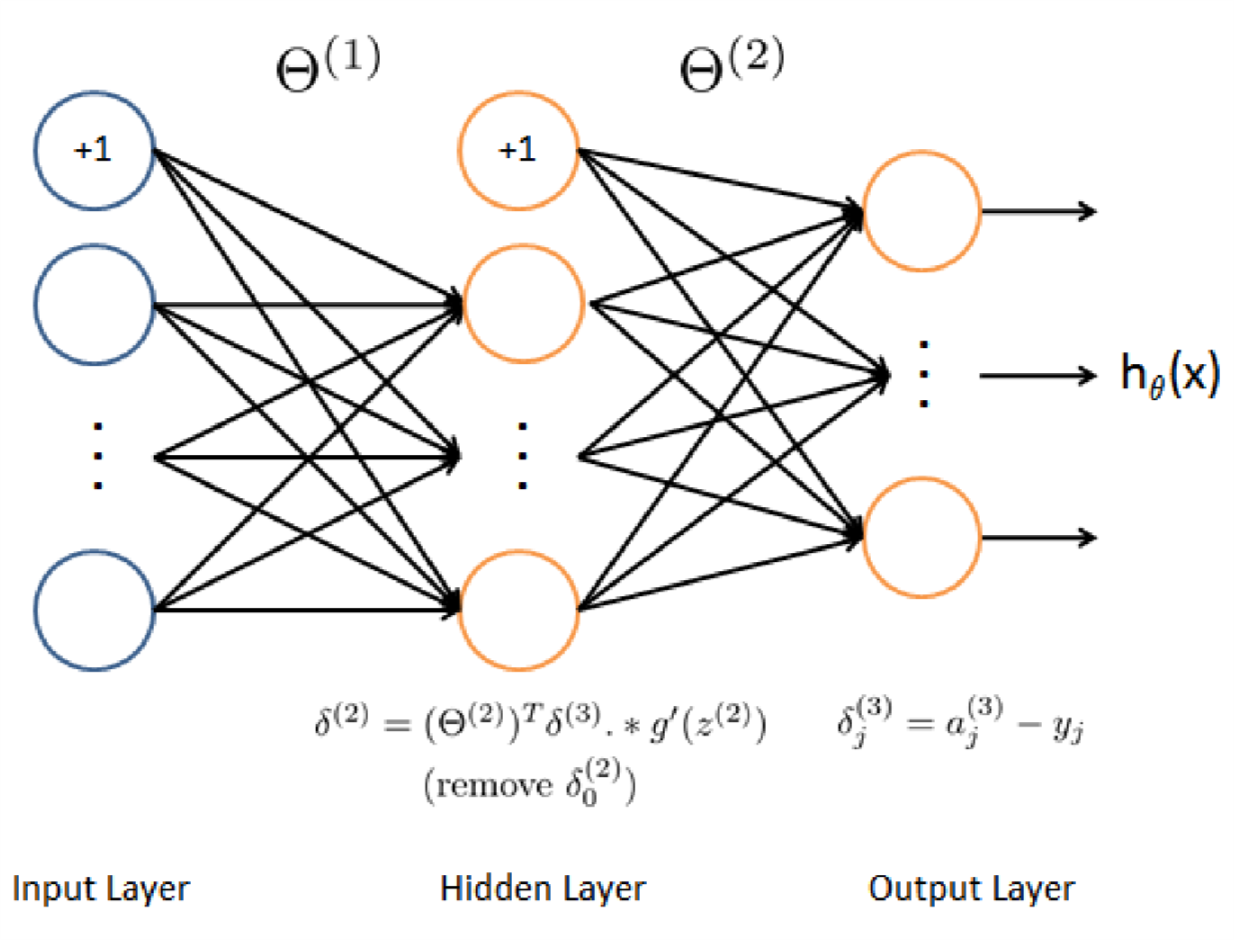
\includegraphics[width=.9\linewidth]{../../img/computer_ng/20171014BPimplement.png}
\end{center}

根据上图,我们需要循环处理所有样本,一次处理一个,所以一定会有一个 \texttt{for t=1:m} 。在第\(t\)次迭代的时候处理第\(t\)个样本。循环内的步骤为:

\begin{enumerate}
\item 设定输入层的值为\(x^{t}\),执行前向过程,计算\(z^{(2)},a^{(2)},z^{(3)},a^{(3)}\)。注意在计算过程中需要为\(a\)添加一个bias项。
\item 对于层3中的每一个输出单元,设定\(\delta_{k}^{(3)} = ( a_{k}^{(3)} - y_{k})\) 其中\(y_{k}\)是二进制数表示当前的训练样本是不是第\(k\)类,如果是,则\(y_{k} = 1\);如果当前样本属于其他类则\(y_{k}=0\)。
\item 对隐藏层\(l=2\),设定:\(\delta^{(2)} = (\Theta^{(2)})^{T}\delta^{(3)}.*g^{'}(z^{(2)})\)
\item 从这个样本中累计梯度值。\[ \Delta^{(l)} = \Delta^{(l)} +\delta^{(l+1)}(a^{(l)})^{T} \] 注意要去掉\(\delta_{0}^{(2)}\)
\item 获得梯度值:\[\frac{\partial}{\partial \Theta_{ij}^{(l)}}J(\Theta) = D_{ij}^{(l)} = \frac{1}{m}\Delta_{ij}^{(l)}\]
\end{enumerate}

在matlab实现的过程中,也需要仔细核对相关变量的维度。由于我们在计算\(a^{(2)},a^{(3)},z^{(2)},z^{(3)}\)的过程中使用的是矢量计算,在计算\(\frac{\partial}{\partial \Theta_{ij}^{(l)}} J(\Theta)\)的过程中我们也可以使用全矢量计算。
\lstset{language=matlab,label= ,caption= ,captionpos=b,numbers=none}
\begin{lstlisting}
%% calculate the theta gradient
delta3 = a3 - Y;
temp = Theta2;
temp(:,1) = 0;
Theta2_grad = delta3 * a2'./m + lambda./m*temp ;

delta2 = Theta2(:,2:end)'*delta3 .* sigmoidGradient(z2);
temp = Theta1;
temp(:,1) = 0;
Theta1_grad = delta2 * a1./m + lambda./m*temp;
\end{lstlisting}
需要注意的是在正则化过程中需要把\(\Theta\)中对应bias项的那些值去掉,在代码中我才用了置零处理。另外在计算\(\delta^{(2)}\)的过程中也需要把\(\Theta_{2}\)中与bias相关的项去掉。
\end{document}
